\documentclass[12pt, letterpaper, twoside]{article}
%\usepackage{epstopdf}
%\usepackage[pdftex]{graphicx}
\usepackage[left=.8in,top=.8in,right=.8in,bottom=.8in,nohead,nofoot,columnsep=20pt]{geometry}
\usepackage{setspace}
\usepackage[small,compact]{titlesec}
\usepackage{subfigure}
\usepackage{multicol}
%\usepackage{multirow}
\usepackage{textcomp}
\usepackage{mathtools}
\usepackage{amsmath}
\usepackage[hyphens]{url}
\usepackage{float}
\usepackage{fancyhdr}
\setlength{\headheight}{14.5pt}
\setlength{\footskip}{11pt}
\pagestyle{fancy}
\lhead{}
\chead{}
\rhead{}
\rfoot{}

\title{Title goes in report.tex}
\author{Bonnie Eisenman, Michael Kranch and Anna Kornfeld Simpson}
\date{COS 597E Software Defined Networks \\ 14 January 2014}

\begin{document}

\maketitle

\begin{spacing}{1.0}

\begin{abstract}
Here's some space for our abstract, which also is in report.tex ... compile this with make in the report directory.  The makefile runs the latex compiler pdflatex 3 times in order to get the references and citations correct; if it says you have undefined references in the output at the end scroll up in the compiler output to find them!
\end{abstract}

\begin{multicols}{2}

\section{Introduction}
We probably want to introduce things, right now that's in report.tex.  We might want to cite something in the introduction, we can do that using \begin{verbatim}{\cite{refname}\end{verbatim} where the \emph{refname} is defined in bibliography.tex in the \begin{verbatim}{\bibitem}\end{verbatim} command.  For example citing dpkt looks like this: \cite{dpkt}.

\section{Related Work}
\label{related}
The related work might be long, so let's put it in a separate file, related.tex
This is related.tex - I've already added all the links from the email thread to the bibliography, we can remove the ones we won't plan to use.
TODO for Anna... look up the two security papers we read in class, add them to the bibliography and talk about them here.


\section{Faking a Switch}
\label{fake}
I'm making up sections and order... there's a file called fake.tex where we can write about faking a switch. The verbatim environment is useful for preformatted text - there's an example in the introduction!
In this section, we present our rogue switch and discuss the protocols necessary to bootstrap communication with the controller.

\subsection {OpenFlow Protocol}
OpenFlow is the protocol used to communicate between the controller and its switches. An OpenFlow packet header is simply an 8 byte packet with the first byte used to communicate version, the second byte for type, third and fourth byte for message length followed by a four byte Transaction ID (see Figure 1). The type is of a subset of 19 possible types, most of which are of type request (e.g. 16 = Stats Request) with the subsequent reply (e.g. 17 = Stats Reply). There are couple key point to note when dealing with the OpenFlow protocol. First, the transaction ID is used to correlate incoming OpenFlow messages with their appropriate responses much in the same way TCP uses SYN and ACK flags. For example, a features reply will (generally) not be accepted by the controller unless it contains the corresponding transaction ID from the features request. This protocol is also a two-way communication scheme and not simply switch replies to controller request. Several message types, to include packet input events, are switch initiated communications to the controller.  

\begin{figure}
  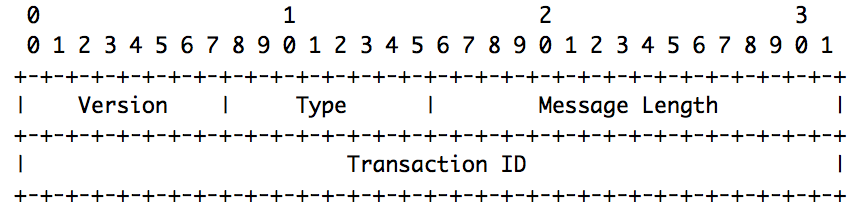
\includegraphics[width=\linewidth]{openflowProtocol.png}
  \caption{OpenFlow Protocol Header Format \cite{protocol}}
  \label{fig:protocol}
\end{figure}

\subsection {Controller Connection Sequence}
While the specific initiation sequence varies by controller, there are several required command to initiate a switch to controller connection\footnote{We specifically tested our rogue switch on the Pox, Ryu and OpenDaylight controllers. Based on our testing and the OpenFlow specifications, we believe all controllers require this small subset of initialization commands but differences might exist based on implementation}. The switch to controller connection simply starts by opening a TCP connection to the controller on the configured port (default 6634)\footnote{As previously discussed, there is no authentication for this connection supported by any tested controller outside of certificate authentication only utilized with OpenVSwitch}.  After opening the connection, the switch sends a Openflow Hello message (0) to the controller. The controller then responds with a Hello message and a Features Request (5) message to which the switch responds with a  Features Reply (6). The controller then sends a Set Config message (9) that does not trigger a reply. Ryu follows this message with a Barrier Request (18), and OpenDaylight follows it with a  Get Config Request (7) to ensure switch configs are set appropriately. OpenDaylight also sends a Flow Modification message (14) to delete any previously installed flows on the switch.

The above commands are all that is needed for the initial controller to switch connection. The switch then proceeds to send several link layer neighbor discovery protocol messages as Packet Input Notification (10) messages to the controller including  Neighbor Solicitation and Router Solicitation messages. The switch also sends a Multicast Listener Report (part of the Multicast Listened Discovery Protocol Version 2) to the controller. Finally, the switch begins periodically (approximately every 3 seconds) sending an OpenFlow Echo Request (2) to the controller as a form of a keep alive with the controller.

\subsection{Our Rogue Switch Utility}
Our Rogue Switch Utility mimics the initial connection sequence to a controller in order to facilitate testing of switch and controller vulnerabilities. Our rogue switch utility does not handle the actual routing of traffic and is instead simply used to disrupt controller and switch traffic flow\footnote{A more advanced utility including routing is discussed in our additional attack section as well as our future work}. The bulk of our utility is a OpenFlow message parser that handles and appropriately responds to controller messages in the correct message format. These messages are generally hardcoded mimicked responses from previously captured live switch communication with minimal dynamic pieces (the transaction id is dynamically assigned for instance)\footnote{Both Pox and Ryu do not actual verify that the transaction ID is correct on most messages. We were able to completely connection to both a Pox and Ryu controller simply my resending previously captured packets. Pox only verifies the transaction id on the Barrier Message of the initial config messages, and this reply can be ignored without the controller ending the TCP session}. 


\section{Disrupting an SDN with a Fake Switch}
\label{attacks}
There's a file called attacks.tex for describing our various attacks; we could combine the results of the attacks we implemented here, or put them separately.
A rogue switch such as we developed could be used for numerous disruptions to SDN functionality or attacks that undermine the security assumptions of the system.  We focused our implementation efforts on exploring the posibility of a denial of service (DOS) or distributed denial of service (DDOS) attack on the controller, and discovered its feasibility across multiple countrollers.  Based on this result and the basic interactions between controller and switch, we outline several other attacks and disruptions. 

\subsection{DOS on the Controller}
We utilized the basic layer 2 MAC address learning example from the Pox and Ryu controllers with a modified the hard flow timeout of 1 as our setup\footnote{We used l2\_learning as our Pox controller and l2\_switch as our Ryu controller.}. We also utilized the basic mininet setup (1 switch with 2 hosts) to test the delay caused by our attack on each controller. To test the delay on the controller, we would simply have h1 ping h2. A more complicated controller (e.g. one that does more than simply add the mac address as a flow) would see its performance decrease more significantly than in our example test cases.

 The first attack we attempted was to see if a single switch could overload the controller by rapidly pushing information. We utilized the basic Echo Request (the switch keep-a-live message) as the OpenFlow message to send to the controller to establish a baseline for testing. Bigger packets, particularly ones that require some sort of computation by the controller application, would increase the performance effect on the controller. We started by sending a Echo Request as quickly as possible to the controller without caring about the response. This attack had little effect of the controller and simply resulted in periodic "TCP Previous Segment Lost" messages as a response from the controller. We believe that the issue with this method was we were never reading in the Echo Replies sent from the controller and the controller was simply ignoring our messages because its send buffer was full. We then modified this attack to send a single Echo Request, wait for an Echo Reply and then instantly send another. This attack caused the controller to continually send Echo Replies but at a controller specified rate - we had to wait for a reply before sending another request. As a result, this attack also had little effect on the controller.

\begin{figure}[ht]
	{\setlength{\fboxsep}{0pt}%
	\setlength{\fboxrule}{1pt}%
	\fbox{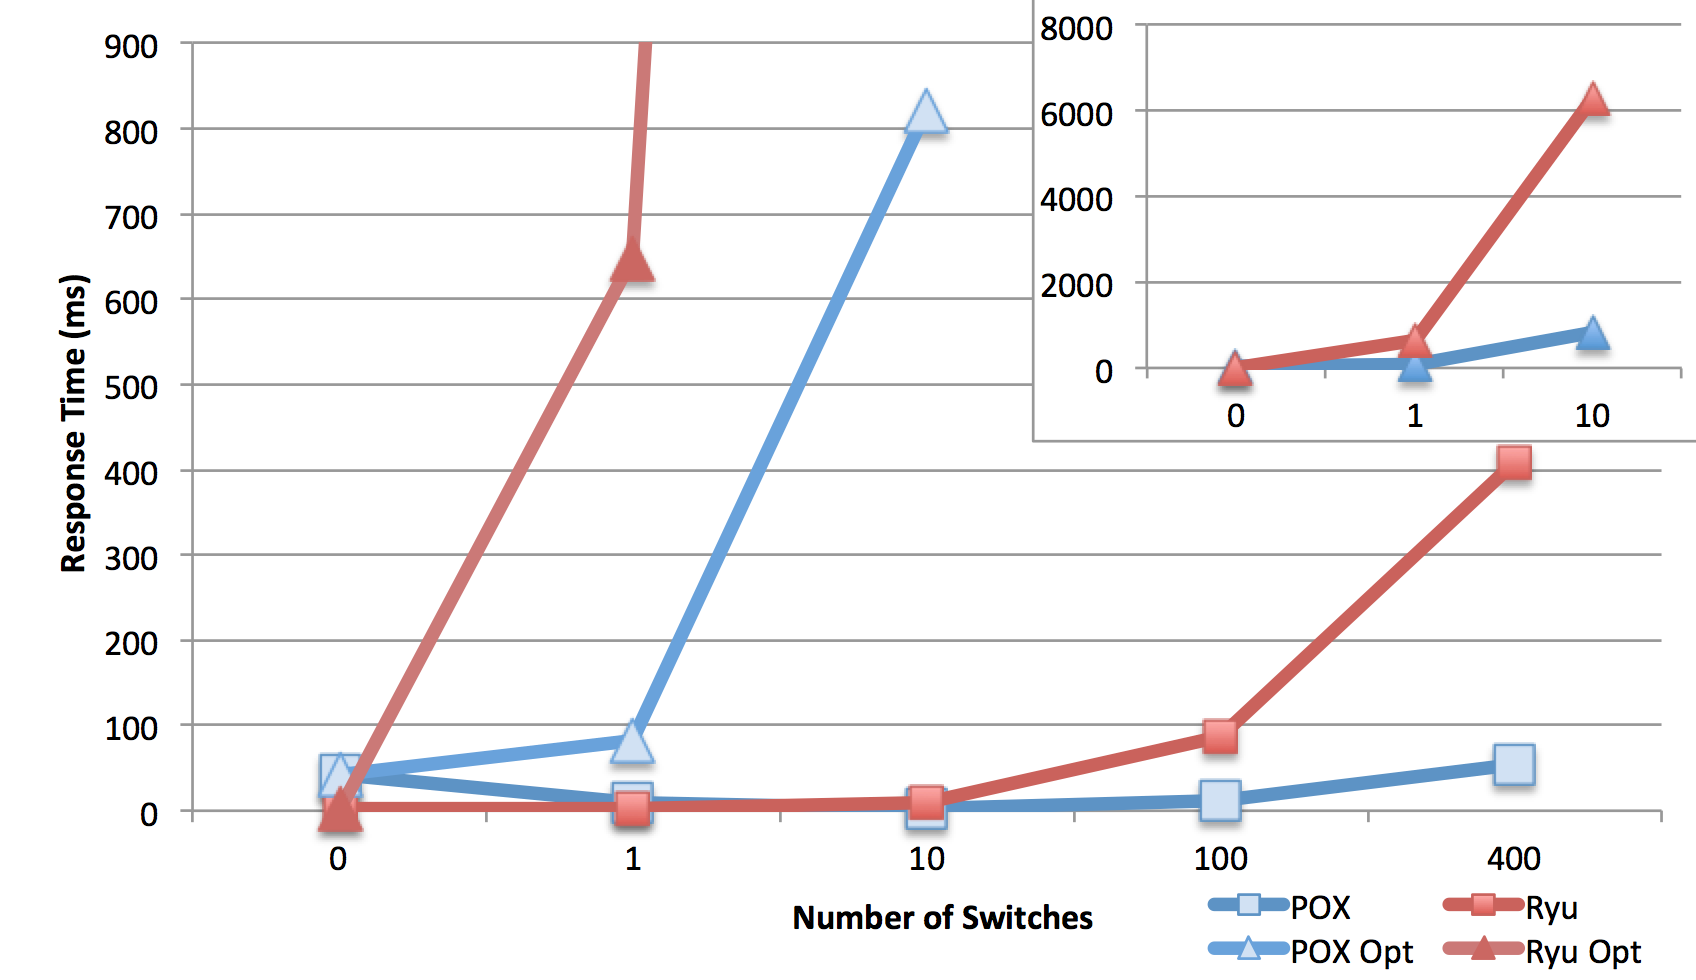
\includegraphics[width=\linewidth]{DOSAttack.png}}
	}%
  \caption{Results of basic and optimized DOS / DDOS on Pox and Ryu Controllers (inset shows expanded view to provide better scale).}
  \label{fig:DOSattacks}
\end{figure}

\subsection{DDoS on the Controller}
   To increase the effect of our attack, we created multiple rogue switches and had each perform the same attack on the controller. Our testing machine was actually the limiting factor in the number of rogue switches we could spawn, but we utilized 400 switches as the max for comparison purposes.  We further optimized our attack by splitting our TCP socket into a distinct listener and sender. We threaded our application so the two actions were not dependent on each other and achieved significantly better results. With out optimized version, we were able to push packets fast enough to cause TCP Window Zero Errors and the controller to have to drop packets.  These results (shown in Figure \ref{fig:DOSattacks}) show that even a single switch can severally effect the performance of a controller and therefore degrade an entire network. 

\subsection{Cloning, dropping, or diverting traffic}

In general, a rogue switch can mishandle packets it receives from the controller or other switches in various ways. Most basically of all, the rogue switch could simply drop packets sent to it, thus creating a service interruption. However, a controller would probably notice this quickly -- it would appear as though the switch had failed, and automated recovery mechanisms would be initiated. More interestingly, a rogue switch could ensure that traffic would be routed through an adversary's middlebox, or could clone traffic and send the cloned stream to the adversary. This would be much more difficult for the controller to detect, unless it caused considerable slowdown. This attack could conceivably be used for purposes such as the NSA's MUSCULAR program, which intercepts traffic as it flows between private data centers \cite{muscular}. 


\subsection{Selective rule modification}
A rogue switch may behave like a normal switch, leading the controller to believe that it is behaving correctly, but then selectively modifying existing rules, ignoring new Flow Mod requests, or adding new ones. For example, dropping packets will be noticed quickly; but a switch could allow packets to pass through that ought to have been dropped. Because of the difficulty of querying flow table state, the controller may not become aware of this. A compromised switch could thus operate in ``stealth mode" and the inconsistent flow table might only be noticed once the switch allows an attacker to pass through, for example.

The switch could also insert its own modifications; for example, it could add VLAN modification rules in order to have malicious traffic be erroneously treated by other network elements. If normal only packets with a certain VLAN tag are allowed to access a sensitive resource, the switch could ensure that the attacker's traffic appears to have valid permissions.

\subsection{Reporting falsehoods to the controller}

A rogue switch can easily send the controller false reports, in order to give the controller an incorrect view of the network state. For example, advertising false host attachments is easy; a rogue switch can send the controller Packet-In events with packets which falsely claim to have a particular MAC address as the sender. This could lead the controller to believe that the compromised switch should receive traffic intended for the host. While this would soon lead to packet loss and a noticeable disruption, it would nevertheless allow a switch to eavesdrop when it would not normally be in a position to do so.

Another potential attack is falsifying measurement reports. When a rogue switch receives a Stats Request, it could respond with a modified Stats Reply that selectively hides or distorts information; for example, making overall traffic levels appear lower so as to disguise a DoS attack. 

The rogue switch could also use the controller as a "relay point" and try to send it Packet In events designed to produce Flow Mods which would then overload other switches' TCAMs or otherwise DoS them. For example, in a MAC learning switch, advertising many new MAC addresses could overload not only the controller, but also other switches, which would have relevant rules installed for the bogus MAC addresses. Thus, instead of attacking each network element individually, the controller gives the attacker an easy, cheap way to concurrently many switches at once. 

\subsection{Learning about the controller}
An adversary could have many reasons to wish to learn more about the controller and the controller's state. By colluding with a rogue switch, the adversary can gain valuable insight into the controller's status.

One possible attack would be for the rogue switch to send Packet In events to the controller and observe the controller's response, in order to determine what kind of applications might be running on the controller. This information could be extremely useful for an attacker who wishes to more narrowly target future attacks.

A more passive attack would be for the rogue switch to relay all observed Flow Mod and Send Packet events received from the controller to an adversary. The adversary could then hope to learn about network traffic or other network events by observing patterns in Flow Mods. Certain Flow Mods might indicate that the controller has, for example, detected an intrusion, or that a specific host has connected to the network in a certain location. To use the MUSCULAR example again, large companies initiate periodical, large-scale data transfers between data centers; this sort of activity would probably cause very predictable Flow Mod messages to be output from the controller, and thus these could be used to determine when a large data transfer was about to take place. Thus, just knowing what Flow Mods are being issued by the controller could be a source of interesting information for an adversary.



\section{Conclusion}
The conclusion might be short enough to be in report.tex - we can add other sections before it as necessary, and the bibliography (in bibliography.tex) will follow.


% Imports the bibliography, don't remove
\small{
\begin{thebibliography}{99}

\bibitem{spymall} Appelbaum et. al. ``Shopping for Spy Gear: Catalog Advertises NSA Toolbox'' \emph{Der Spiegel} 29 December 2013 \url{www.spiegel.de/international/world/catalog-reveals-nsa-has-back-doors-for-numerous-devices-a-940994.html}

\bibitem{benton} Benton et. al. ``OpenFlow Vulnerability Assessment'' \emph{ACM SIGCOMM Hot Topics in Software Defined Networking (HotSDN)}, 2013. 

\bibitem{ethane} Casado et. al. ``Ethane: Taking Control of the Enterprise'' \emph{ACM SIGCOMM}, 2007.

\bibitem{sane} Casado et. al. ``SANE: A Protection Architecture for Enterprise Networks'' \emph{USENIX Security Symposium}, 2006.

\bibitem{cisco} Cisco. ``Multiple Vulnerabilities in Cisco TelePresence Multipoint Switch'' 11 July 2012 \url{tools.cisco.com/security/center/content/CiscoSecurityAdvisory/cisco-sa-20120711-ctms}

\bibitem{ciscopatch} Constantin, Lucian. ``Cisco patches vulnerabilities in some security applications, switches, and routers.'' \emph{InfoWorld} 10 October 2013, \url{http://www.infoworld.com/d/security/cisco-patches-vulnerabilities-in-some-security-appliances-switches-and-routers-228551}

%\bibitem{dpkt} dugsong et. al. ``dpkt'' \url{code.google.com/p/dpkt}

\bibitem{history} Feamster et. al. ``An Intellectual History of Programmable Networks.'' \emph{ACM Queue} 2013.

\bibitem{muscular} Gellman et. al. ``How we know the NSA had access to internal Google and Yahoo cloud data'' \emph{Washington Post, The Switch}, 4 November 2013, \url{http://www.washingtonpost.com/blogs/the-switch/wp/2013/11/04/how-we-know-the-nsa-had-access-to-internal-google-and-yahoo-cloud-data/}

\bibitem{4d} Greenberg et. al. ``A clean-slate 4D approach to network control and management.'' \emph{ACM SIGCOMM Computer Communications Review}, 2005.

\bibitem{nox} Gude et. al. ``NOX: Towards an operating system for networks'' \emph{ACM SIGCOMM Computing Communication Review}, 2008.

%\bibitem{hecker} Hecker, Artur. ``Carrier SDN: Security and Resilience Requirements'' 15 November 2013 \url{http://www.ikr.uni-stuttgart.de/Content/itg/fg524/Meetings/2013-11-15-Muenchen/12_ITG524_Muenchen_Hecker.pdf}

\bibitem{onix} Koponen et. al. ``Onix: a distributed control platform for large-scale production networks.'' \emph{USENIX Symposium on Operating Systems Design and Implementation (OSDI)}, 2010.

\bibitem{sdnsec} Kreutz et. al. ``Towards Secure and Dependable Software-Defined Networks'' \emph{ACM SIGCOMM HotSDN}, 2013.

\bibitem{openflow} McKeown et. al. ``OpenFlow: Enabling innovation in campus networks'' \emph{ACM SIGCOMM Computer Communication Review}, 2008.

\bibitem{resonance} Nayak et. al. ``Resonance: dynamic access control in enterprise networks'' \emph{ACM Workshop on Research on Enterprise Networking}, 2009.

\bibitem{opendaylight} Open Daylight, 2013-2014. \url{http://www.opendaylight.org}

\bibitem{protocol} ``OpenFlow Packet Protocol.'' \emph{OpenFlow}, \url{archive.openflow.org/wk/images/c/c5/Openflow_packet_format.pdf}

\bibitem{openvswitch} Pfaff et. al. ``Extending Networking into the Virtualization Layer'' \emph{ACM Workshop on Hot Topics in Networks (HotNets)}, 2009.

\bibitem{pox} POX developers. \url{http://www.noxrepo.org/pox/about-pox}

%\bibitem{pycap} Rowe, Mark. ``Python Packet Capture and Injection Library'' \url{pycap.sourceforge.net}

\bibitem{ryu} ``Ryu SDN framework'' \url{http://osrg.github.io/ryu}

\bibitem{attacking} Shin and Gu. ``Attacking Software-Defined Networks: A First Feasibility Study (Extended Abstract)'' \emph{ACM SIGCOMM HotSDN}, 2013.

%\bibitem{tcqack} Stretch, Jeremy. ``Understanding TCP Sequence and Acknowledgement Numbers'' 7 June 2010, \url{http://packetlife.net/blog/2010/jun/7/understanding-tcp-sequence-acknowledgment-numbers/}

\end{thebibliography}
}


\end{multicols}

\end{spacing}

\end{document}
